\subworkpkg{1.1}

%% Tasks

%% A. Search for 5 existing (or planned) similar missions and identify
%% for these missions:

%% a. the mission objectives and, if possible, the associated mission
%% requirements;

%% b. the main elements that make up the mission and their main
%% function(s);

%% c. the main performance and design characteristics of these
%% elements.

%% B. Define the mission elements with which the design process will
%% interact (e.g.: mission operations, ground system, launch system,
%% etc.).

%% C. List the main objectives to be achieved in the design process
%% (related to, e.g., payload capability, performance, structure,
%% etc.). Mention at least 10 objectives.

%% D. For each one of the identified design objectives, list the main
%% functionalities that the design must provide in order to accomplish
%% it.

%% E. List all the design parameters that are already available (e.g.,
%% from the project description provided in Section 3) and the ones
%% which still need to be identified.

%% Deliverables

%% D1.1.1. Comparative table including all the relevant information
%% collected for the reference missions identified under Task A above.

\deliverable{1.1.1}

\begin{longtable}{ll}
  \caption{Similar missions.} \\

  Mission & Launch date \\

  Galileo & October 1989 \\

  Juno & August 2011 \\

  Jupiter Europa Orbiter (JEO) & February 2020 \\

  Jupiter Icy Moon Explorer (JUICE) & 2022 \\

  Cassini & October 1997 \\
\end{longtable}

\begin{longtable}{p{\textwidth}}
  \caption{Similar missions' objectives and associated requirements}
  \\

  Galileo \\* \midrule

  \begin{itemize}
  \item Study Jupiter’s atmosphere, satellites, and magnetosphere by
    deploying a Jupiter orbiter and conducting various experiments.
  \item Send a probe to the surface of Jupiter to identify atmospheric
    materials and conditions that cannot be detected from outside.
  \item Venus and Earth flyby for extensive survey on the planets’
    surface and atmosphere (including imaging)
  \end{itemize}

  Requirements. Durable spacecraft and orbiter. Safe transmission of
  the data to Earth.  Strongly built probe which can survive
  penetration of the atmosphere as well as ground impact and operate
  without malfunctions.

  Juno \\* \midrule

  \begin{itemize}
  \item Observe Jupiter's gravity and magnetic fields, atmospheric
    dynamics and composition. Thus, ultimately, investigate the
    formation and evolution of Jupiter.
  \end{itemize}

  Requirements. Durable spacecraft with maneuverability. Safe
  transmission of the data to Earth. \\

  JEO \\* \midrule

  \begin{itemize}
  \item Europa’s Ocean: Characterize the extent of the ocean and its
    relation to the deeper interior
  \item Europa’s Ice Shell: Characterize the ice shell and any
    subsurface water, including their heterogeneity, and the nature of
    surface-ice-ocean exchange
  \item Europa’s Chemistry: Determine global surface compositions and
    chemistry, especially as related to habitability
  \item Europa’s Geology: Understand the formation of surface
    features, including sites of recent or current activity, and
    identify and characterize candidate sites for future in situ
    exploration
  \item Jupiter System: Understand Europa in the context of the
    Jupiter system
  \end{itemize} \\

  JUICE \\* \midrule

  \begin{itemize}
  \item To characterize the conditions that may have led to the
    emergence of habitable environments among the Jovian icy
    satellites, with special emphasis on the three ocean bearing
    worlds, Ganymede, Europa, and Callisto
  \end{itemize}

  Requirements. 2 flybys of Europa, 12 flybys of Callisto. Orbit
  around Ganymede, Optimal illumination conditions and high pointing
  accuracy for high-resolution imaging. Different orbits possible. A
  minimum average downlink of 1.4Gb/day \\

  Cassini \\* \midrule

  \begin{itemize}
  \item Bring the Huygens probe to Saturn’s moon Titan.
  \item Study the moons Titan and Encladus as well as the other icy
    moons
  \end{itemize} \\ \bottomrule
\end{longtable}

\begin{longtable}{p{\textwidth}}
  \caption{Similar missions' main elements and their main functions}
  \\ \toprule

  Galileo \\* \midrule

  \begin{itemize}
  \item Launch (aboard a Space Shuttle). Achieve escape velocity from
    Earth and to head for Jupiter
  \item Release from the Space Shuttle and the provision of the
    thrust.
  \item Flying past the Moon, Venus and several asteroids. Carry out
    observation and imaging.
  \item Sending the probe into Jupiter's atmosphere. Identify
    atmospheric constituents and conditions that cannot be detected
    from outside.
  \item Sending the orbiter into Jovian orbit. Observe the surface,
    atmosphere, and magnetosphere of the Jupiter.
  \item Termination of the mission by plunging into Jupiter's
    atmosphere.
  \end{itemize} \\

  Juno \\* \midrule

  \begin{itemize}
  \item Launch (aboard a Space Shuttle). Achieve Earth escape velocity
    and head for Jupiter.
  \item Release from the Space Shuttle and the provision of thrust.
  \item Earth flyby for gravity assist.
  \item Flight to Jupiter and arrival into Jovian orbit.
  \end{itemize} \\

  JEO \\* \midrule

  \begin{itemize}
  \item Launch (aboard a Space Shuttle Atlas V 551). Achieve Earth
   escape velocity and head for Jupiter.
  \item Release from the Space Shuttle and the provision of thrust.
  \item Venus and Earth flyby for gravity assist.
  \item Flight to Jupiter, and Jovian orbit insertion.  insertion
  \item Transfer to Europa orbit (Europa orbit insertion) followed by
    science mapping phase.
  \item Termination of the mission. Impact the surface of Europa after
    running out of fuel.
  \end{itemize} \\

  JUICE \\* \midrule

  \begin{itemize}
  \item Launch by Ariana-5 ECA
  \item Cruise. Interplanetary transfer from Earth to Jupiter.
  \item Jupiter tour. A transfer to Callisto, 2 Europa and 3 Callisto
    flybys, Jupiter high latitude phase, including 9 Callisto flybys,
    and finally a transfer to Ganymede.
  \item Ganymede tour, consisting of elliptical and high altitude
    circular phases, 500km altitude orbit and a 200km altitude orbit.
  \item End of mission.
  \end{itemize} \\

  Cassini \\* \midrule

  \begin{itemize}
  \item Launch.
  \item Jupiter flyby to provide the final push for the trajectory to
    Saturn and to study Jupiter from two different spacecraft at the
    same time.
  \item Release of the Huygens probe to Titan.
  \item Start extended mission in which different moons of Saturn are
    studied.
  \end{itemize} \\ \bottomrule
\end{longtable}

\begin{longtable}{p{\textwidth}}
  \caption{Similar missions' main performance and design
    characteristics} \\ \toprule

  Galileo \\* \midrule

  \begin{itemize}
  \item Launch Vehicle. Space Shuttle Atlantis (STS-34R)
  \item The spacecraft's propulsion module consists of twelve
    10-newton (2.25-pound-force) thrusters and a single 400-newton
    (90-pound-force) engine which use monomethylhydrazine fuel and
    nitrogen-tetroxide oxidizer
  \item Spacecraft Instruments.
    \begin{itemize}
    \item Orbiter instruments. Imaging system. Near-infrared mapping
      spectrometer. Ultraviolet spectrometer.
      Photopolarimeter-radiometer. Magnetometer. Energetic-particles
      detector. Plasma detector. Plasma wave and heavy ion
      counter. Radio system
    \item Atmospheric entry probe instruments. Atmospheric structure
      instrument.  Neutral mass spectrometer. Helium abundance
      detector. Net flux
      radiometer. Nephelometer. Lightning/energetic-particles
      experiment.
    \end{itemize}
  \item Spacecraft Power. Two Radioisotope Thermoelectric Generators.
  \item Antenna Diameter. 4.8-meter.
  \end{itemize} \\

  Juno \\* \midrule

  \begin{itemize}
  \item Launch Vehicle. Atlas V551
  \item Fuel Mass. 1,280 kilograms of fuel and 752 kilograms of
    oxidizer.
  \item Spacecraft Instruments. Gravity Science Experiment.
    Magnetometer, Microwave Radiometer. Particle Detector. Jovian
    Infrared Auroral Mapper (JIRAM). Ultraviolet Imaging Spectrograph
    (UVS).
  \item Spacecraft power. Solar Arrays. Dimensions of each solar array
    29.5 feet (9 meters) by 8.7 feet (2.65 meters).
  \item Propulsion. Dual mode propulsion subsystem. Bi-propellant main
    engine and mono-propellant reaction control system thrusters. The
    12 reaction control system thrusters allow translation and
    rotation about three axes.
  \item Command and Data Handling. A RAD750 flight processor with 256
    megabytes of flash memory and 128 megabytes of DRAM local
    memory. Provides 100 Mbps total instrument throughput.
  \item Power. Power generation is provided by three solar arrays
    consisting of 11 solar panels and one MAG boom.
  \end{itemize} \\

  JEO \\* \midrule

  \begin{itemize}
  \item Launch Vehicle. Atlas V551.
  \item Radiation shielding to protect electronic components and
    assemblies.
  \item Telecommunications. 3m HGA with a 2-axis gimbal. 25 W X-band
    and Ka-band TWTAs.
  \item Attitude control. 3-axis stabilized with reaction wheels and
    coupled thrusters.
  \item Power. 540W RPS (MMRTG or ASRG). Lithium Ion battery for peak
    power management.
  \item Propulsion. Bi-propellant, 900N engine.
  \item Spacecraft instruments. Laser Altimeter (LA). Radio Science
    (RS). Ice Penetrating Radar (IPR).  VIS-IR Imaging Spectrometer
    (VIRIS).  UV Spectrometer (UVS).  Ion and Neutral Mass,
    Spectrometer (INMS).  Thermal Instrument (TI).  Narrow Angle
    Camera (NAC).  Wide Angle Camera and Medium, Angle Camera
    (WAC+MAC).  Magnetometer (MAG).  Particle and Plasma Instrument
    (PPI).
  \end{itemize} \\

  JUICE \\* \midrule

  \begin{itemize}
  \item 3-axis stabilized.
  \item Power. Solar panels. 636-693W (EOM).
  \item High Gain Antenna. 3.2 m. Body fixed.
  \item X and Ka bands. Downlink > 1.4 Gbit/day.
  \item High delta-V capability (2700 m/s).
  \item Radiation level. 240krad/10 mm Al solid sphere.
  \item Dry mass at launch. ~1800kg.
  \end{itemize} \\

  Cassini \\* \midrule

  \begin{itemize}
  \item 3-axis stabilized.
  \item 2,150 kg orbiter.
  \item 350kg probe.
  \item 3,132kg fuel.
  \item 3 radioisotope thermoelectric generators for 880W. 670W left
    in 2010.
  \end{itemize} \\
\end{longtable}

\begin{longtable}{ll}
  \caption{Sources.} \\ \toprule

  Galileo & \cite{galileonasa,galileojpl} \\

  Juno & \cite{junonasa} \\

  JEO & \cite{jeonasa} \\

  JUICE & \cite{juiceesa} \\

  Cassini & \cite{cassininasa} \\ \bottomrule
\end{longtable}

%% D1.1.2. Block diagram showing the outcomes of Task B above (hint:
%% you can put the item to be designed in the middle, and the relevant
%% mission elements around it).

\deliverable{1.1.2}

The design will have to interact with the following mission elements.

\begin{figure}[h]
  \caption{Mission elements.}
  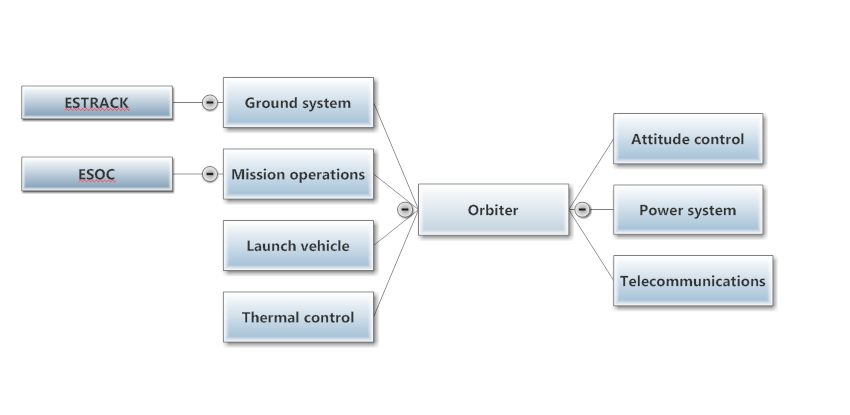
\includegraphics[width=\textwidth]{block-diagram-WP1-1B}
\end{figure}

\begin{itemize}
\item{Ground system.} The ground segment will use ESTRACK.
\item{Mission operations.} The mission operations center will be ESOC.
\item{Launch vehicle.}
\item{Thermal control.}
\item{Attitude control.}
\item{Power system.}
\item{Telecommunications.}
\item{Radiation shielding.}
\item{Propulsion systems.}
\item{S/C structures.}
\item{Orbit / trajectory}
\end{itemize}

%% D1.1.3. Numbered lists obtained from Tasks C, D and E above (note:
%% lists should be as complete as it is possible at this stage of the
%% design, and a clear justification for each listed item shall be
%% provided).

\deliverable{1.1.3}

The following mission objectives must be met

\begin{enumerate}
\item{Payload size.} \SI{0.7}{m} x \SI{0.7}{m} x \SI{0.7}{m}
\item{Payload orientation.} Free View for Camera, etc.
\item{$\Delta V$ budget.} To be determined.
\item{Power requirements.} Maximum payload power: \SI{50}{W}
\item{Payload operational temperature.} \SI{150}{K}--\SI{200}{K}
\item{Lifetime.} More than 3 years.
\item{Data storage and transfer.} To be determined.
\item{Reliability.} At least 0.9.
\item{Shielding (radioactive radiation).} To be determined.
\end{enumerate}

The already known design parameters are

\begin{enumerate}
\item{Payload mass.} \SI{80}{kg}
\item{Payload dimensions.} \SI{0.7}{m} x \SI{0.7}{m} x \SI{0.7}{m}
\item{Payload required power.} \SI{50}{W}
\item{Payload operational temperature range.} \SI{150}{K}--\SI{200}{K}
\item{Orbit.} Polar, \SI{200}{km} above Europa surface.
\item{Mission duration.} At least 3 years in Europa orbit.
\item{Launch date.} Around 2020.
\item{Total mission cost.} Less than 500 million FY2000 USD.
\item{Mission reliability.} 0.9.
\end{enumerate}

The design parameters yet to be determined include

\begin{enumerate}
\item{Radiation environment and shielding.} Radiation levels demand adequate
  shielding.
\item{$\Delta V$ budget.}
\item{Payload orientation.} Free field of view for instruments.
\item{Data storage and transfer.}
\end{enumerate}
